% =====================================================================
% IE643 LATENT NAVIGATORS — POSTER VERSION 9
% Revised from V5 in response to presentation feedback:
%   balanced section spacing, explanatory text, consecutive figure
%   numbers 1-6, a clearer conclusion, and six focused references.
%   V8 restores the full cat degradation severity grid in Figure 3.
% Print: ISO A1 portrait (594 x 841 mm), XeLaTeX.
% =====================================================================
\documentclass[a1,portrait]{a1poster}
\usepackage{fontspec}
\setmainfont{Liberation Serif}
\usepackage{graphicx,amsmath,amssymb,booktabs,array,xcolor,tikz,hyperref}
\usetikzlibrary{calc}
\hypersetup{hidelinks,pdftitle={Latent Navigators IE643 Poster - Version 9},pdfauthor={Ananna Biswas}}
\graphicspath{{figures/}}
\definecolor{Navy}{HTML}{183B65}
\definecolor{DeepGreen}{HTML}{23563F}
\definecolor{Ink}{HTML}{22272B}
\definecolor{Gray}{HTML}{5F6973}
\definecolor{Thin}{HTML}{BBC4CE}
\pagestyle{empty}
\setlength{\parindent}{0pt}
\setlength{\parskip}{0pt}
\newcommand{\Pbody}{\fontsize{17.3}{22.0}\selectfont\color{Ink}}
\newcommand{\Psmall}{\fontsize{15.6}{20.0}\selectfont\color{Ink}}
\newcommand{\Psmaller}{\fontsize{14.4}{18.5}\selectfont\color{Ink}}
\newcommand{\Pcaption}{\fontsize{13.0}{16.4}\selectfont\color{Gray}}
\newcommand{\Pref}{\fontsize{10.8}{13.3}\selectfont\color{Ink}}
\newcommand{\puttext}[4]{\node[anchor=north west,inner sep=0pt] at (#1,-#2) {\begin{minipage}[t]{#3mm}\raggedright #4\end{minipage}};}
\newcommand{\headat}[3]{\node[anchor=north west,inner sep=0pt,text=Ink,font=\bfseries\fontsize{32.0}{37}\selectfont] at (#1,-#2) {#3};}
\newcommand{\smhead}[3]{\node[anchor=north west,inner sep=0pt,text=Navy,font=\bfseries\fontsize{19.5}{23}\selectfont] at (#1,-#2) {#3};}
\begin{document}
\begin{tikzpicture}[remember picture,overlay,x=1mm,y=1mm]
\begin{scope}[shift={(current page.north west)},xshift=25mm,yshift=28mm]

% ===================== ORIGINAL INSTRUCTOR HEADER =====================
\node[anchor=north west,inner sep=0pt] at (25,-22) {
\includegraphics[width=66mm,height=75mm,keepaspectratio]{logo.png}};
\node[anchor=north east,inner sep=0pt] at (568,-22) {
\includegraphics[width=66mm,height=75mm,keepaspectratio]{IE643-Logo.pdf}};
\node[anchor=north,text=DeepGreen,font=\bfseries\fontsize{33}{37}\selectfont] at (297,-16) {IE643 Course Project};
\node[anchor=north,text=Navy,font=\bfseries\fontsize{40}{44}\selectfont,align=center,text width=414mm] at (297,-45) {Classification in Class-Imbalanced\\Extremely Shifted Images};
\node[anchor=north,text=Navy,font=\bfseries\fontsize{23}{27}\selectfont] at (297,-93) {Latent Navigators};
\node[anchor=north,text=Ink,font=\fontsize{19}{22}\selectfont] at (297,-109) {Ananna Biswas (25M1727)};
\node[anchor=north,text=Ink,font=\fontsize{16.5}{19.5}\selectfont] at (297,-121) {25m1727@iitb.ac.in};
\draw[Navy,line width=1.08mm] (21,-138) rectangle (573,-829);
\draw[Navy,line width=.53mm] (297,-147) -- (297,-734);
\draw[Thin,line width=.36mm] (30,-734) -- (564,-734);
\draw[Thin,line width=.36mm] (30,-785) -- (564,-785);

% ========================= LEFT COLUMN =========================
\headat{33}{147}{Abstract}
\puttext{33}{175}{251}{\Pbody
This project studies image classification and object localization when rare objects appear under poor visibility. I built an imbalanced 10-class PASCAL VOC dataset and tested clean and shifted images. ResNet-50 predicts image-level labels; YOLOv8n predicts object boxes. My proposed clean-anchored, minority-aware YOLO training raises clean detection mAP@0.5 from \textbf{0.664 to 0.734} and severe low-light mAP from \textbf{0.015 to 0.058}.}

\headat{33}{222}{Introduction}
\puttext{33}{249}{251}{\Pbody
\textbf{Problem:} most training examples belong to common classes, while bicycle, motorbike, bus, boat and cat are less frequent. Darkness, haze and adverse weather also hide object features.\\[0.8mm]
\textbf{Why deep learning?} CNNs learn visual features and multi-scale detectors locate objects. My goal is to improve minority-class robustness \emph{while keeping clean-image performance strong}.}

\headat{33}{286}{Workflow}
\node[anchor=north west,inner sep=0pt] at (34,-314) {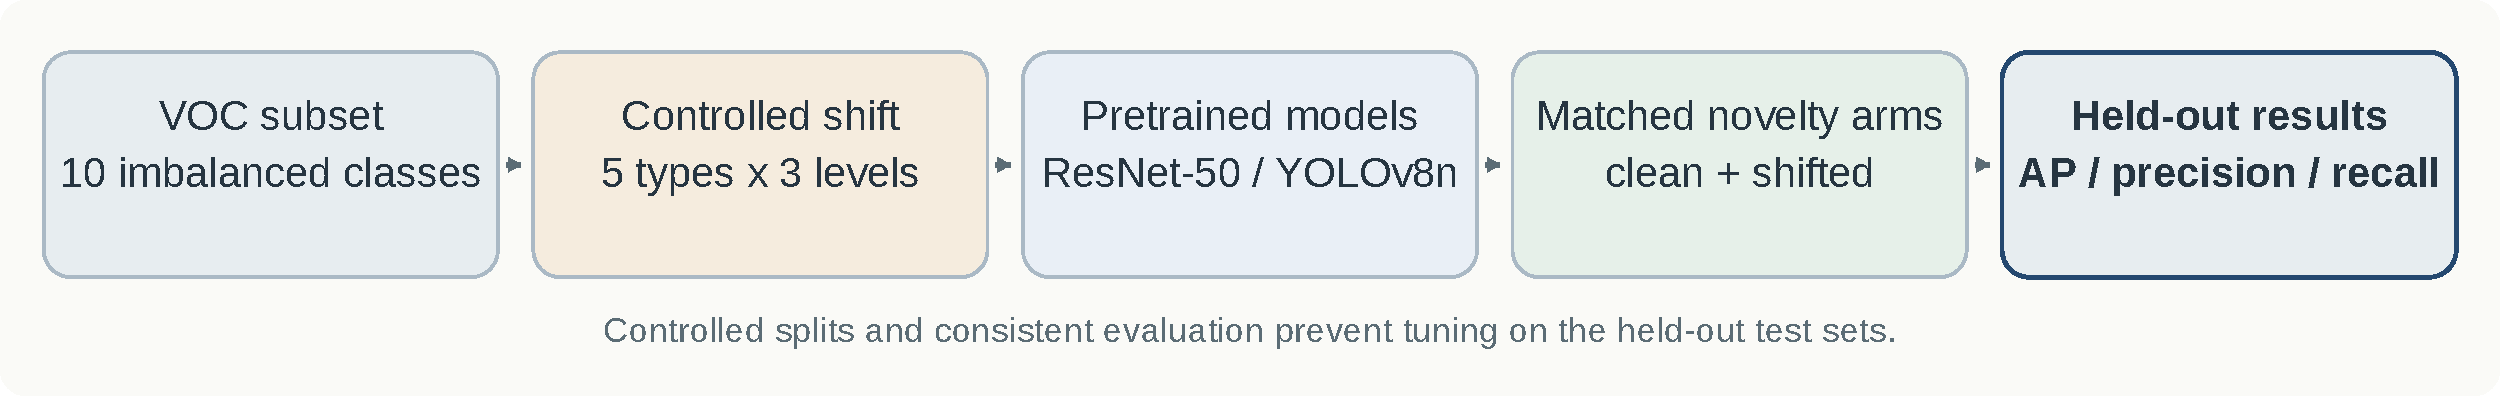
\includegraphics[width=249mm]{workflow_v9.pdf}};
\puttext{35}{358}{247}{\Pcaption \textbf{Figure 1.} Project workflow: data preparation, baseline training, controlled novelty experiments and held-out evaluation.}

\headat{33}{379}{Methods and Approaches}
\puttext{33}{406}{250}{\Psmall
My framework contains \textbf{two deep-learning branches} (Figure 2): ResNet-50 for multi-label classification and YOLOv8n for object detection. Both start from pretrained weights; the novelty changes YOLO's training strategy, not its network layers.}
\node[anchor=north west,inner sep=0pt] at (34,-432) {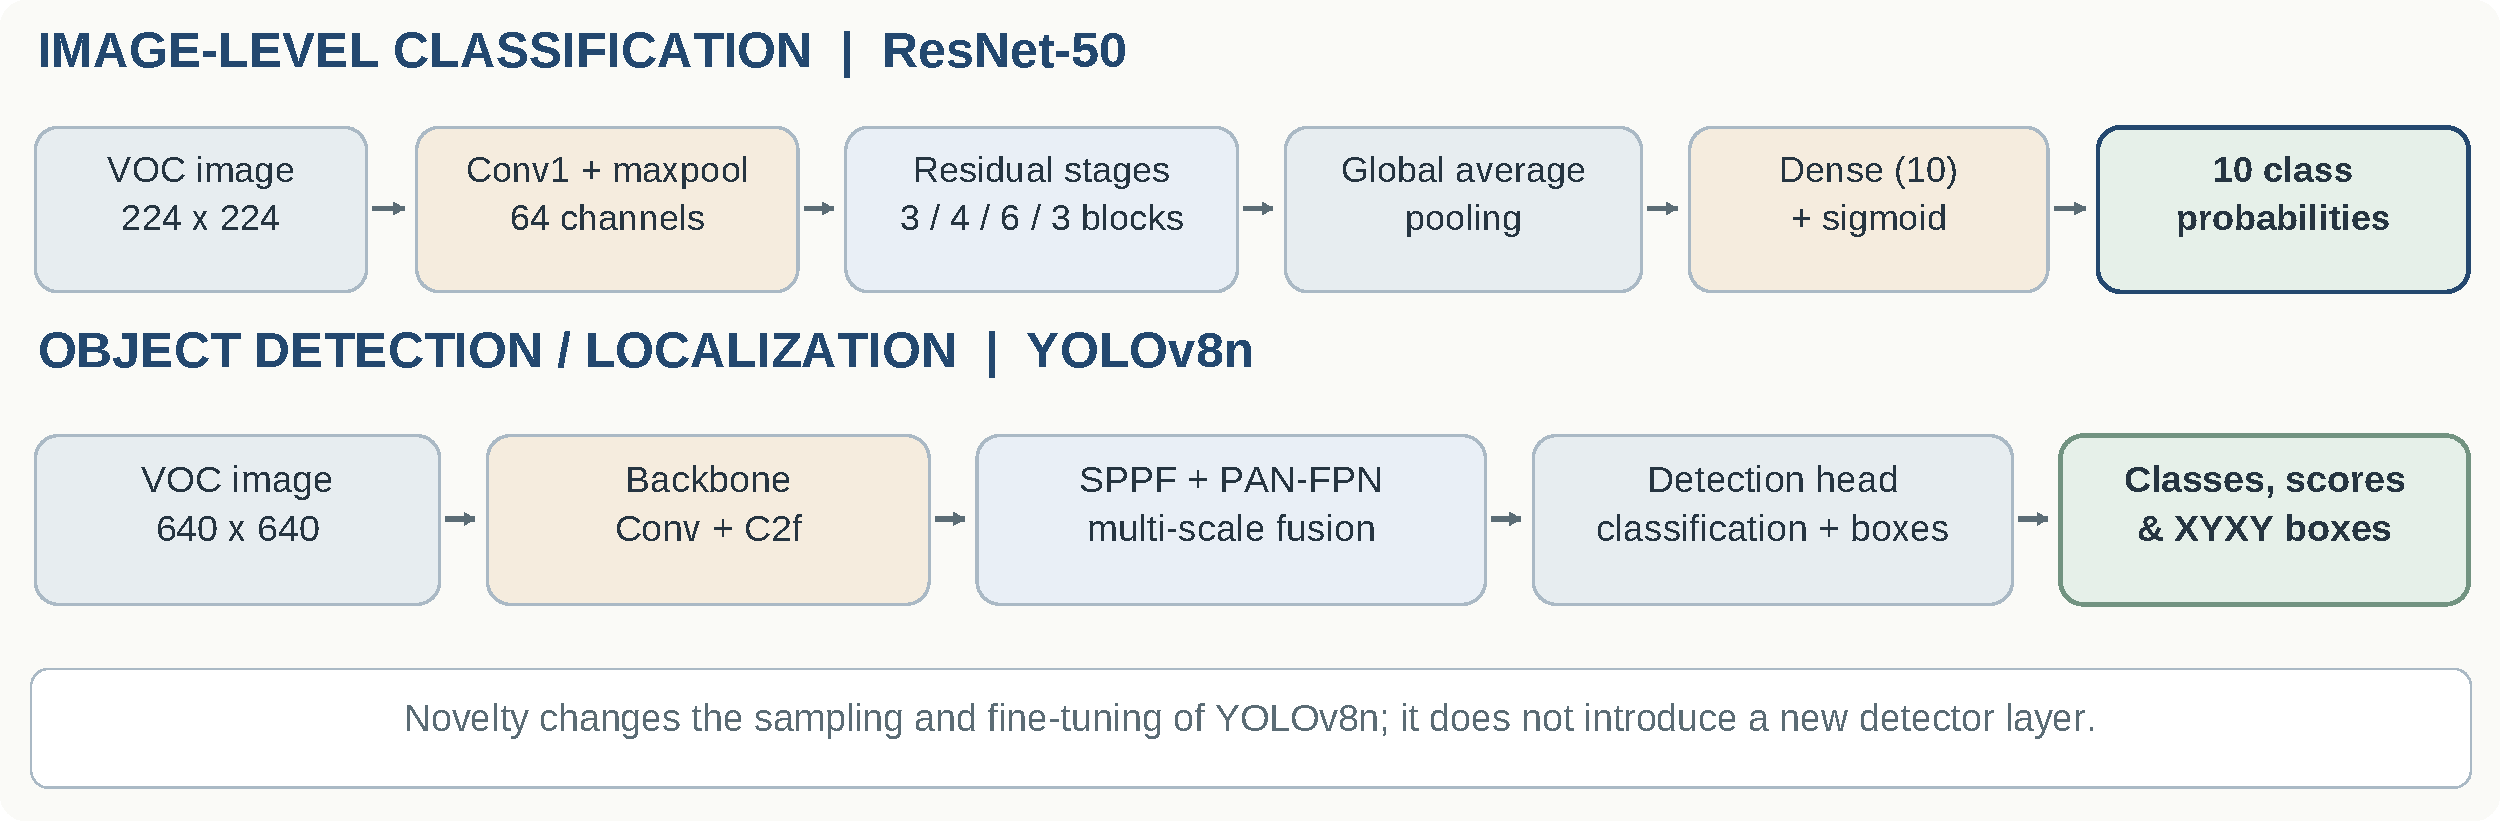
\includegraphics[width=237mm]{combined_architecture_v9.pdf}};
\puttext{35}{516}{247}{\Pcaption \textbf{Figure 2.} Combined architecture: residual CNN features for classification; backbone, neck and detection head for localization.}
\puttext{34}{533}{249}{\Psmaller
\textbf{Classification:} ResNet-50 produces 10 sigmoid scores and uses weighted binary cross-entropy. Effective-number weighting, $E_c=(1-\beta^{n_c})/(1-\beta)$ with $\beta=0.999$, gives a normalized bicycle weight of \textbf{12.54} (30 bicycle versus 463 person images) [2].\\[0.4mm]
\textbf{Detection:} pretrained YOLOv8n [4] has a backbone, neck and multi-scale detection head. Novelty changes fine-tuning, \emph{not} its network layers.}

\headat{33}{568}{Dataset Details}
\puttext{33}{589}{251}{\Psmaller
\textbf{Training data:} 1,176 clean VOC images; five majority classes (person: 463 positives) and five minority classes (30 positives each). Figure 3 shows five corruptions at three severity levels.}
\puttext{35}{612}{248}{\fontsize{12.9}{15.5}\selectfont\color{Ink}
\renewcommand{\arraystretch}{0.98}
\begin{tabular}{@{}p{105mm}p{59mm}p{75mm}@{}}\toprule
\textbf{Evaluation data} & \textbf{Size} & \textbf{Purpose}\\\midrule
VOC test & 4,823 images & Clean reference\\
VOC synthetic & 5 shifts $\times$ 3 & Controlled robustness\\
ExDark / RTTS / DAWN & 2,563 / 3,674 / 873 & Natural shifts\\\bottomrule
\end{tabular}}
\node[anchor=north west,inner sep=0pt] at (46,-644) {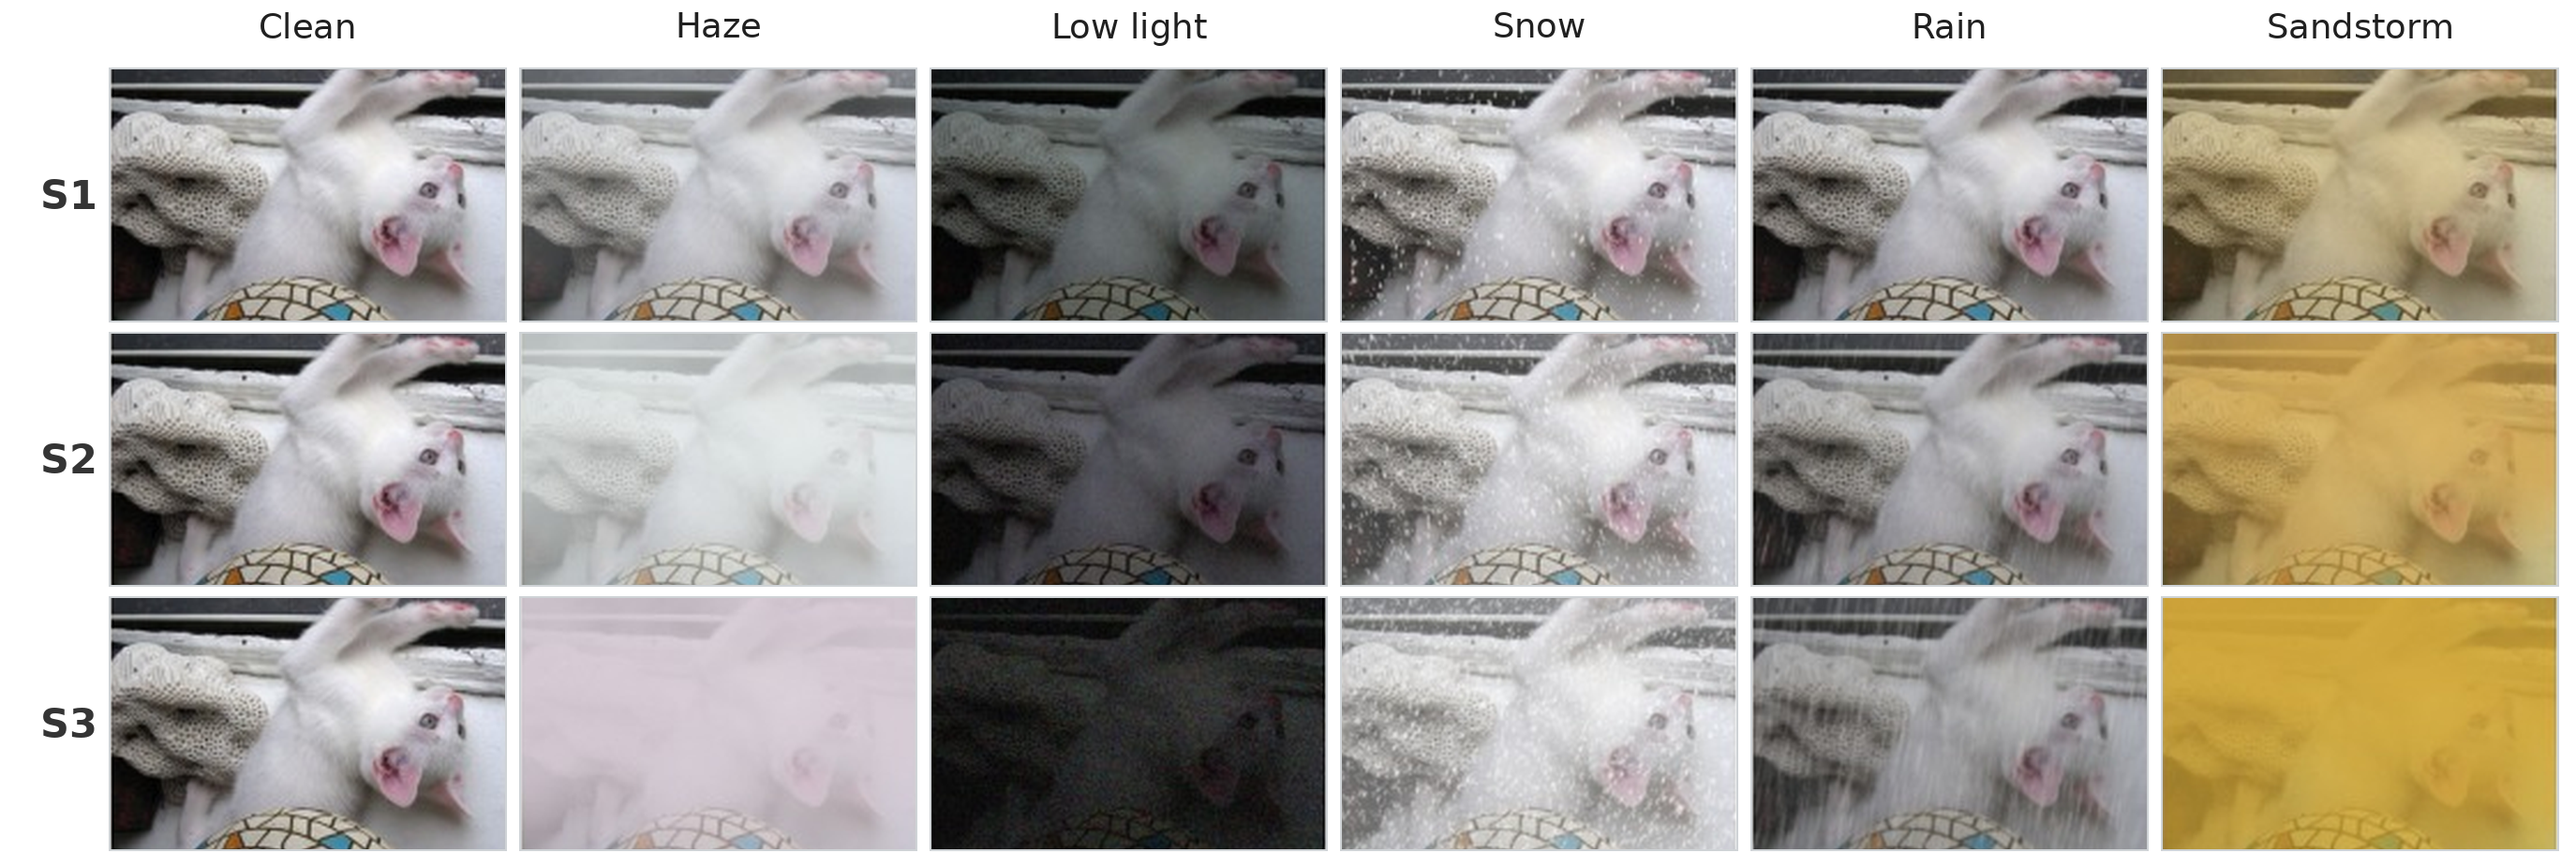
\includegraphics[width=220mm]{cat_corruption_severity_v8.png}};
\puttext{35}{721}{248}{\Pcaption \textbf{Figure 3.} The same cat under haze, low light, snow, rain and sandstorm at severity levels 1--3 (S1--S3). Stronger shifts make the object less visible.}

% ========================= RIGHT COLUMN ========================
\headat{309}{147}{Novelty Assessment}
\puttext{309}{175}{251}{\Pbody
\textbf{Earlier problem:} the combined YOLO model improved some corrupted conditions but reduced clean VOC mAP from 0.664 to 0.643. Severe low light was especially difficult. I therefore kept all clean images in training and gave more attention to minority examples under low-light shifts.}
\node[anchor=north west,inner sep=0pt] at (311,-213) {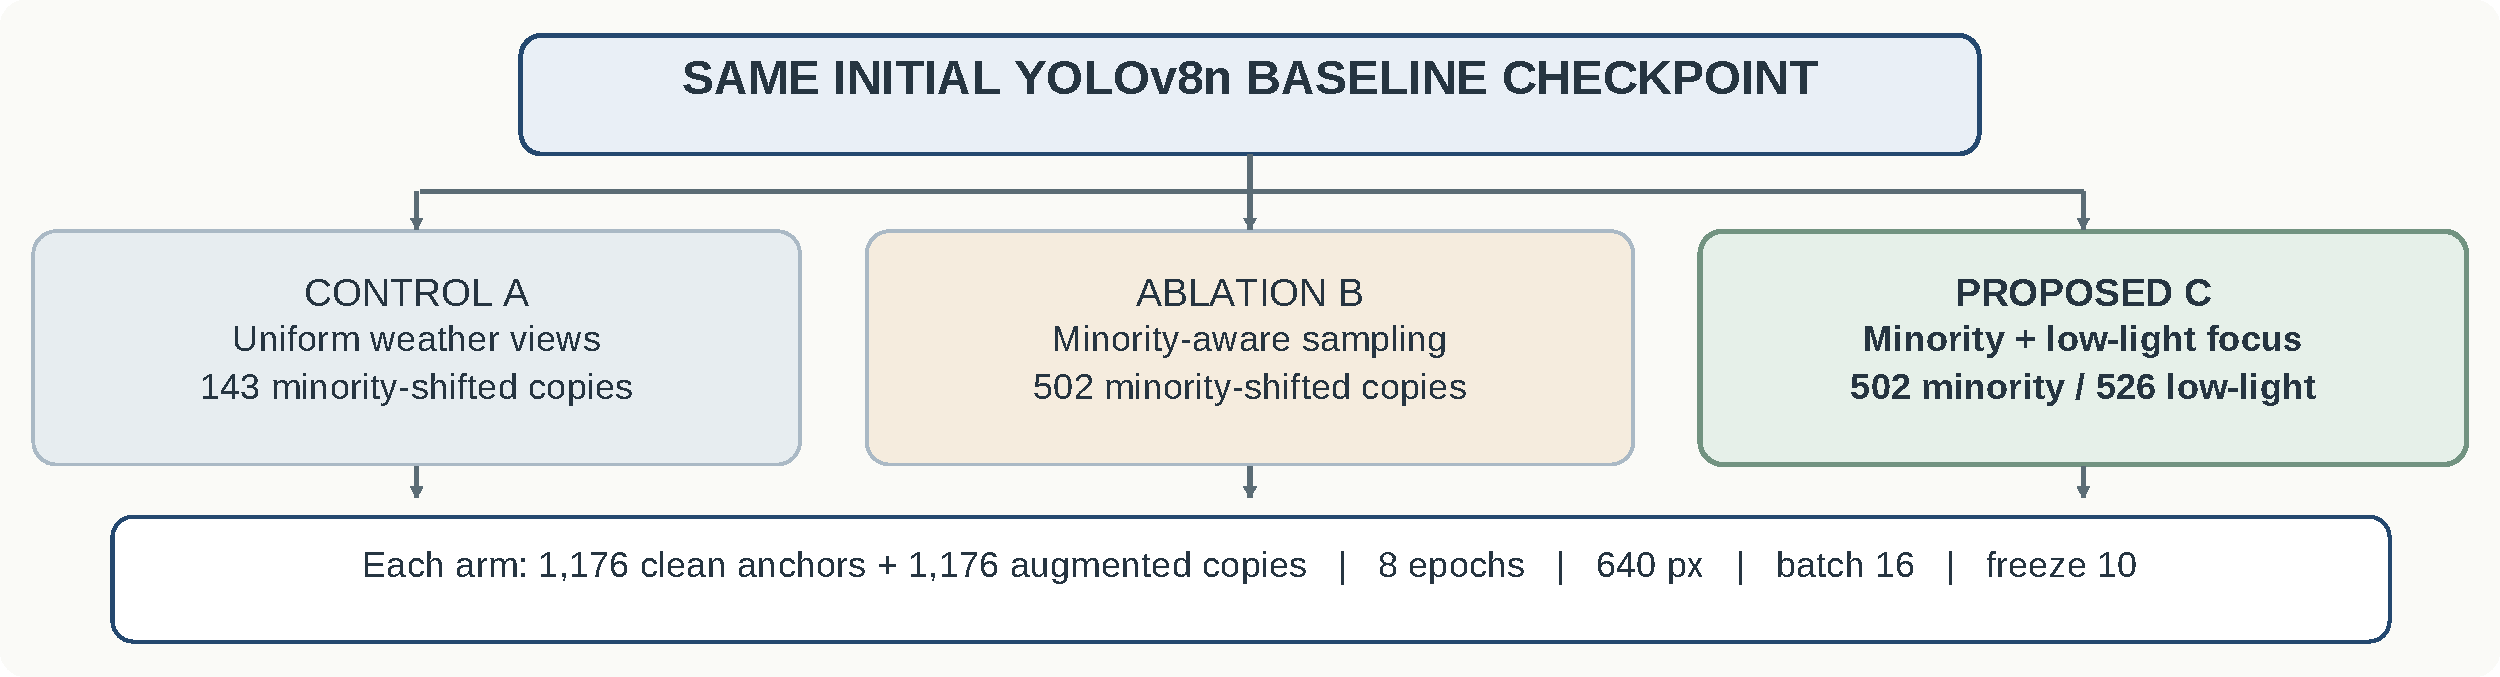
\includegraphics[width=238mm]{novelty_arms_v9.pdf}};
\puttext{310}{289}{250}{\Pcaption \textbf{Figure 4.} Controlled ablations: uniform augmentation, minority sampling, and the proposed minority-plus-low-light strategy.}
\puttext{310}{309}{251}{\Psmall
\textbf{Fair comparison:} each arm had 1,176 clean and 1,176 corrupted views, using the same starting checkpoint, 8 epochs, image size 640, batch 16, frozen first 10 layers and $lr_0=2\times10^{-4}$. Proposed sampling upweights minority images by a factor of five.}
\puttext{310}{346}{251}{\Psmaller
\textbf{Checkpoint choice:} on separate VOC tuning images, shift scores were 0.178 (uniform), 0.192 (minority sampling) and \textbf{0.196 (proposed)}. A clean-accuracy safeguard was applied before held-out testing.}

\headat{309}{369}{Results}
\puttext{310}{395}{251}{\Psmaller
\textbf{Earlier classification ablation:} minority synthetic mAP was 0.653 at baseline, 0.706 with weighting, and 0.817 with weighting plus augmentation. Clean classification mAP rose from 0.796 to 0.808.}
\node[anchor=north west,inner sep=0pt] at (310,-420) {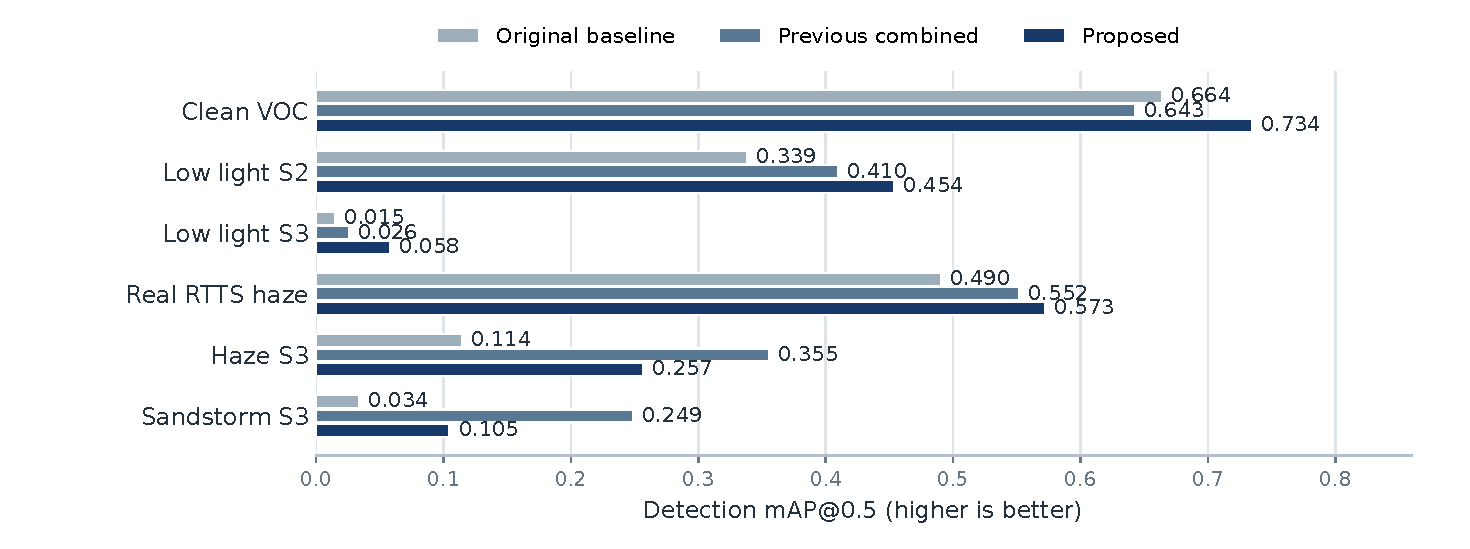
\includegraphics[width=215mm]{heldout_chart_v5.pdf}};
\puttext{310}{506}{251}{\Pcaption \textbf{Figure 5.} YOLOv8n held-out detection mAP@0.5: baseline, previous combined model, and proposed model; higher is better.}
\smhead{310}{532}{Minority-class detection recall}
\puttext{311}{546}{248}{\Psmaller
\renewcommand{\arraystretch}{1.06}
\begin{tabular}{@{}p{105mm}rrr@{}}\toprule
\textbf{Condition} & \textbf{Baseline} & \textbf{Prior} & \textbf{Proposed}\\\midrule
Clean VOC & 0.495 & 0.557 & \textbf{0.607}\\
Low light S3 & 0.126 & 0.052 & \textbf{0.232}\\
Real RTTS haze & 0.282 & \textbf{0.420} & 0.369\\\bottomrule
\end{tabular}}
\smhead{310}{593}{Qualitative results}
\node[anchor=north west,inner sep=0pt] at (311,-613) {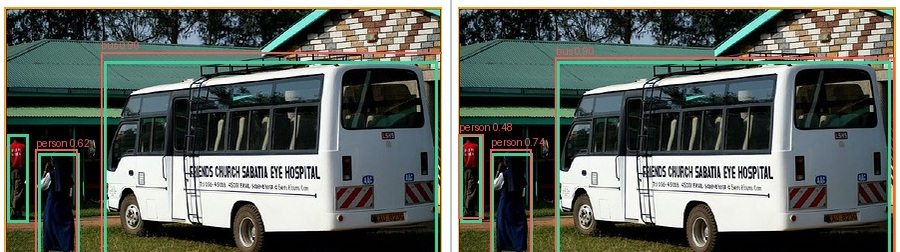
\includegraphics[width=169mm]{qualitative_clean_cropped_v5.jpg}};
\puttext{310}{666}{250}{\Pcaption \textbf{Figure 6.} Clean VOC: baseline versus proposed. Low-light diagnostic misses: 22 vs. 18 (12 images; not full recall).}

\headat{309}{682}{Conclusions and Future Work}
\puttext{310}{706}{251}{\Psmaller
Clean-anchored, minority-aware tuning improved clean VOC mAP and recall, and helped severe low light. It did not outperform the earlier combined model in extreme haze or sandstorm, and RTTS minority recall was lower. Robustness is therefore shift-dependent. Future work will test multi-weather sampling, inspect box-location errors and repeat training with several random seeds.}

% ======================== REFERENCES + FOOTER =========================
% Six focused sources relevant to the networks, loss, dataset, software and adverse weather.
\headat{33}{739}{References}
\puttext{33}{762}{251}{\Pref
[1] K. He, X. Zhang, S. Ren and J. Sun. \emph{Deep Residual Learning for Image Recognition}. CVPR, 2016. \href{https://arxiv.org/abs/1512.03385}{arxiv.org/abs/1512.03385}.\\[0.3mm]
[2] Y. Cui, M. Jia, T.-Y. Lin, Y. Song and S. Belongie. \emph{Class-Balanced Loss Based on Effective Number of Samples}. CVPR, 2019. \href{https://arxiv.org/abs/1901.05555}{arxiv.org/abs/1901.05555}.\\[0.3mm]
[3] M. Everingham et al. \emph{The PASCAL Visual Object Classes (VOC) Challenge}. IJCV, 2010. \href{https://doi.org/10.1007/s11263-009-0275-4}{doi.org/10.1007/s11263-009-0275-4}.}
\puttext{309}{762}{252}{\Pref
[4] G. Jocher, A. Chaurasia and J. Qiu. \emph{Ultralytics YOLOv8}, software repository. \href{https://github.com/ultralytics/ultralytics}{github.com/ultralytics/ultralytics}. Accessed 24 Nov. 2026.\\[0.3mm]
[5] C. Michaelis et al. \emph{Benchmarking Robustness in Object Detection: Autonomous Driving when Winter is Coming}. arXiv, 2019. \href{https://arxiv.org/abs/1907.07484}{arxiv.org/abs/1907.07484}.\\[0.3mm]
[6] B. Li et al. \emph{Benchmarking Single Image Dehazing and Beyond}. IEEE TIP, 2019. \href{https://arxiv.org/abs/1712.04143}{arxiv.org/abs/1712.04143}.}

% ----- Footer: demo QR verified; GitHub QR reserved for later. -----
\node[anchor=north west,inner sep=0pt,text=Ink,font=\bfseries\fontsize{17.5}{21}\selectfont] at (32,-791) {Acknowledgements};
\node[anchor=north west,inner sep=0pt,text=Ink,font=\bfseries\fontsize{17.5}{21}\selectfont] at (130,-791) {Link to github repo};
\node[anchor=north west,inner sep=0pt,text=Ink,font=\bfseries\fontsize{17.5}{21}\selectfont] at (310,-791) {Link to Demo video};
\puttext{32}{808}{96}{\Pcaption I thank Prof. P. Balamurugan (course instructor) and the TAs for their guidance.}
\IfFileExists{figures/github_qr.png}{\node[anchor=north west,inner sep=0pt] at (240,-788) {\href{https://github.com/ananna-b/IE643-Latent-Navigators}{
\includegraphics[width=36mm,height=36mm]{github_qr.png}}};}{\draw[Gray,densely dashed,line width=.3mm] (240,-788) rectangle (276,-824);\node[align=center,text=Gray,font=\fontsize{11}{13}\selectfont] at (258,-806) {GitHub QR\\placeholder};}
\IfFileExists{figures/demo_qr.png}{\node[anchor=north west,inner sep=0pt] at (520,-788) {\href{https://drive.google.com/drive/folders/1WqmOQDdKV1TnngI-oDce9uJfPOYvQpE4?usp=sharing}{
\includegraphics[width=36mm,height=36mm]{demo_qr.png}}};}{\draw[Gray,densely dashed,line width=.3mm] (520,-788) rectangle (556,-824);\node[align=center,text=Gray,font=\fontsize{11}{13}\selectfont] at (538,-806) {Demo QR\\placeholder};}
\end{scope}
\end{tikzpicture}
\null
\end{document}
